\documentclass[a4paper,11pt,titlepage]{jsarticle}

\usepackage{amsmath}
\usepackage{amssymb}
\usepackage{amsfonts}
\usepackage{bm}
\usepackage[dvipdfmx]{graphicx}
\usepackage{listings}
% \usepackage{jvlisting}
% \usepackage{jlisting}
\usepackage{otf}
\usepackage{float}
\usepackage{url}
\usepackage{ascmac}
\usepackage{fancybx}
% \bibliographystyle{junsrt} % スタイル(番号順)
% \bibliographystyle{plain}
% \bibliography{references}  % references.bib を指定(拡張子は不要)

\lstset{%ソースコードの表示に関する設定
    basicstyle={\ttfamily},
    identifierstyle={\small},
    commentstyle={\smallitshape},
    keywordstyle={\small\bfseries},
    ndkeywordstyle={\small},
    stringstyle={\small\ttfamily},
    frame={tb},
    breaklines=true,
    columns=[l]{fullflexible},
    numbers=left,
    xrightmargin=0zw,
    xleftmargin=3zw,
    numberstyle={\scriptsize},
    stepnumber=1,
    numbersep=1zw,
    lineskip=-0.5ex
}

% 画像ファイルを検索するディレクトリを指定
\graphicspath{ {images/} }
%これを設定しておけば,自動的にimages/から画像を参照してくれる。
%================================

\begin{document}

\title{知能情報実験 \ajroman{3}(データマイニング班)\\顔画像に基づく美男美女の識別と一般人との比較による特徴抽出}
\author{215706D:KIM HYUNWOO, 235221E:山脇大輝,\\ 235701B:松田遼平, 235732B:長\UTF{7028}一生}
\date{提出日: 2025年7月18日}
\maketitle

\tableofcontents
\clearpage

\begin{abstract}
本グループでは、美男美女(有名人)と一般人を分類する機械学習システムを構築した。美男美女ランキングから対象者の顔写真をスクレイピングで収集し、一般人データとのバランスを図るため前処理を実施した。前処理として画像サイズ調整や顔位置の正規化を行い、分類器を構築した。実験では美男美女と一般人の顔画像の識別を試み、機械学習モデルから人間の美的感覚に近い判断をどの程度行えるかというデータを明らかにする。
\end{abstract} 


\section{はじめに}
\subsection{実験の目的と達成目標(アプローチの全体像を含む)}
本グループでは「顔画像データを用いて、一般的に“美男美女”と称される有名人と一般人を識別・分類し、特徴差を明らかにすること」をテーマとして設定した。

人の美しさや魅力は主観的に表されることが多く,機械学習を用いて客観的に分析することを試みる。fairfaceのモデル構築の際に用いられた画像群と独自に美男美女の画像から構築したデータセットを用いて,画像認識のための深層学習モデルであるResNet18, ResNet34, ResNet50とEfficientNet\_b0を用いて,美男美女(有名人)と称される顔写真と一般人の写真を識別・分類するモデルの構築を問題として設定した。最終的には,有名人と一般人の差から美しさや魅力度合いがどのように違うのかを定量化・可視化し,美的評価の要素を客観的に明らかにする。また,人の美しさは黄金比や対称性といった要素で評価されることが多いが,モデルが人間の美的感覚に近い判断をどの程度行えるかというデータを明らかにする.

\subsection{意図していた実験計画との違い}
fairfaceには,データセットと学習済みモデルの2種類が公開されているが,当初の調べ不足が原因でデータセットのみと勘違いして実験計画を立てていた。fairfaceでは,すでに画像収集・前処理・ResNet34による分析まで行い高精度を叩き出している。これらと同様のことを本実験で行っても車輪の再開発となり実験の意義は少ない。そこでfairfaceに追加学習を行うことにした。fairfaceに用意されているデータセットに加え,独自にデータセットを構築し,さらに有名人・一般人のラベル付をした画像を学習することで意義深い実験ができることを志した。


\section{実験方法}
\subsection{実験目的}
世界で美男・美女(有名人)と呼ばれる人の顔写真と一般人の顔写真を分類するモデルを作り,美男・美女と一般人の分類を行う。

\subsection{データセット構築・前処理}
有名人と一般人を分類するモデルを構築するために,2つのデータセットを準備し,前処理を行い,モデルの学習・評価を行う。

\subsubsection{FairFaceとは}
本実験ではFairFaceというモデルを用いて,分類評価を行うと同時に,独自構築した分類モデルも作成した。ここで,FairFaceというモデルについて概要を説明すると,従来の多くの顔画像データセットでは,特定の人種(白人)や性別にデータの偏りが見られる傾向にある。FairFaceでは,7つの人種グループ:白人、黒人、インド人、東アジア人、東南アジア人、中東人、ラテンアメリカ人でデータ数を均一して,人種差の少ないデータセット構築を行った。これにより,機械学習モデルの特定の人種・性別への偏り・バイアスの軽減を実現した顔画像データセット及びモデルである。
構築されたデータセットについては,主に大規模なパブリックデータセットyahoo YFCC100M(Flickr画像)から、意図的に人種バランスを考慮したサンプリング手法を用いて収集され、加えてTwitterやオンライン新聞からの画像も含まれている。YFCC100M全体からランダムに顔画像をサンプリングし,各国の人口構成を推定し,データセットが特定(白人)の人種に偏らないように画像数を調節した。これにより他の人種を過小評価するデータセットのバイアスを軽減している。


\subsubsection{定義}
本実験では,以下のように一般人と有名人の定義を行う。
\begin{itemize}
    \item 一般人:fairfaceのデータセットで作成されたデータセット。
    \item 有名人:2024年度世界の美男美女ランキング上位top50を有名人として定義する。
\end{itemize}

\subsubsection{データセット構築}
\begin{itemize}
    \item 一般人のデータセット:FairFaceのデータセットを使用
    \item 美男・美女のデータセット:独自構築を行った。
        \begin{itemize}
            \item[(1)] 美男・美女の基準を決定 \\
                \cite{bidanshi}や\cite{bijoshi}より2024年度美男美女ランキングtop50を美男美女として扱う
            \item[(2)] データの収集 \\
                対象者の画像は,「2024年度美男美女ランキング」top50の人名からbing検索エンジンを用いてwebスクレイピングした。
                \begin{itemize}
                    \item ソースコードを以下のGitHubにて公開する。
                    \item \url{https://github.com/e235221/info3dm_racial_classification}
                \end{itemize}
        \end{itemize}
\end{itemize}
    
\subsubsection{前処理}
\begin{itemize}
    \item リサイズ
        \begin{itemize}
            \item 収集したデータの顔部分だけ切り取り,サイズを$300 \times 300$とし,FairFaceのデータセットと合わせて調整する.
        \end{itemize}
    \item 正面・側面の判定
        \begin{itemize}
            \item 顔の向きが学習に与える影響を排除するために,hopenetを用いて正面を向いている画像のみ抽出した。側面を向いている画像はデータセットから除外している。
            \item HopeNetとは,1枚の顔写真からYaw(左右の向き),Pitch(上下の向き),Roll(傾き)を求め,その人がどの方向を向いているのかを推定する深層学習モデルである。感情認識などに用いられている。
        \end{itemize}
    \item アップサンプリング・ダウンサンプリング
        \begin{itemize}
            \item アップサンプリング:データ数の少ない美男美女データの各画像を左右反転させることでデータ数を2倍に増やした。
            \item ダウンサンプリング:データ数の多い有名人データセットからランダムにデータを削除することで,有名人データセットと一般人データセットのデータ件数を調節した。
            \item 画像数については,trainで31000枚ずつ,testで7800枚ずつの画像を用意した。
        \end{itemize}
    \item 美男美女・一般人データセットに対して,ラベル付け
        \begin{itemize}
            \item webスクレイピングしで収集した画像データに対して,fairfaceで用意されているラベル付けと同様に美男美女データセットに対してもラベル付けを行い,それに加えて一般人か有名人かを判別するためにそれぞれ0と1を付与した。
            \item 新規作成した美男美女データセットについては,手作業で検索し,国籍・誕生日のラベルを付与した。
            \item \texttt{file\_name,age,gender,race,0/1}の5種類を列名としてcsvを作成した。\texttt{file\_name}に指定されたpathで画像を読み込み,学習を行う。
        \end{itemize}
    \item ファイルのリネーム
\end{itemize}


%======================
\begin{figure}[H]
    \centering
    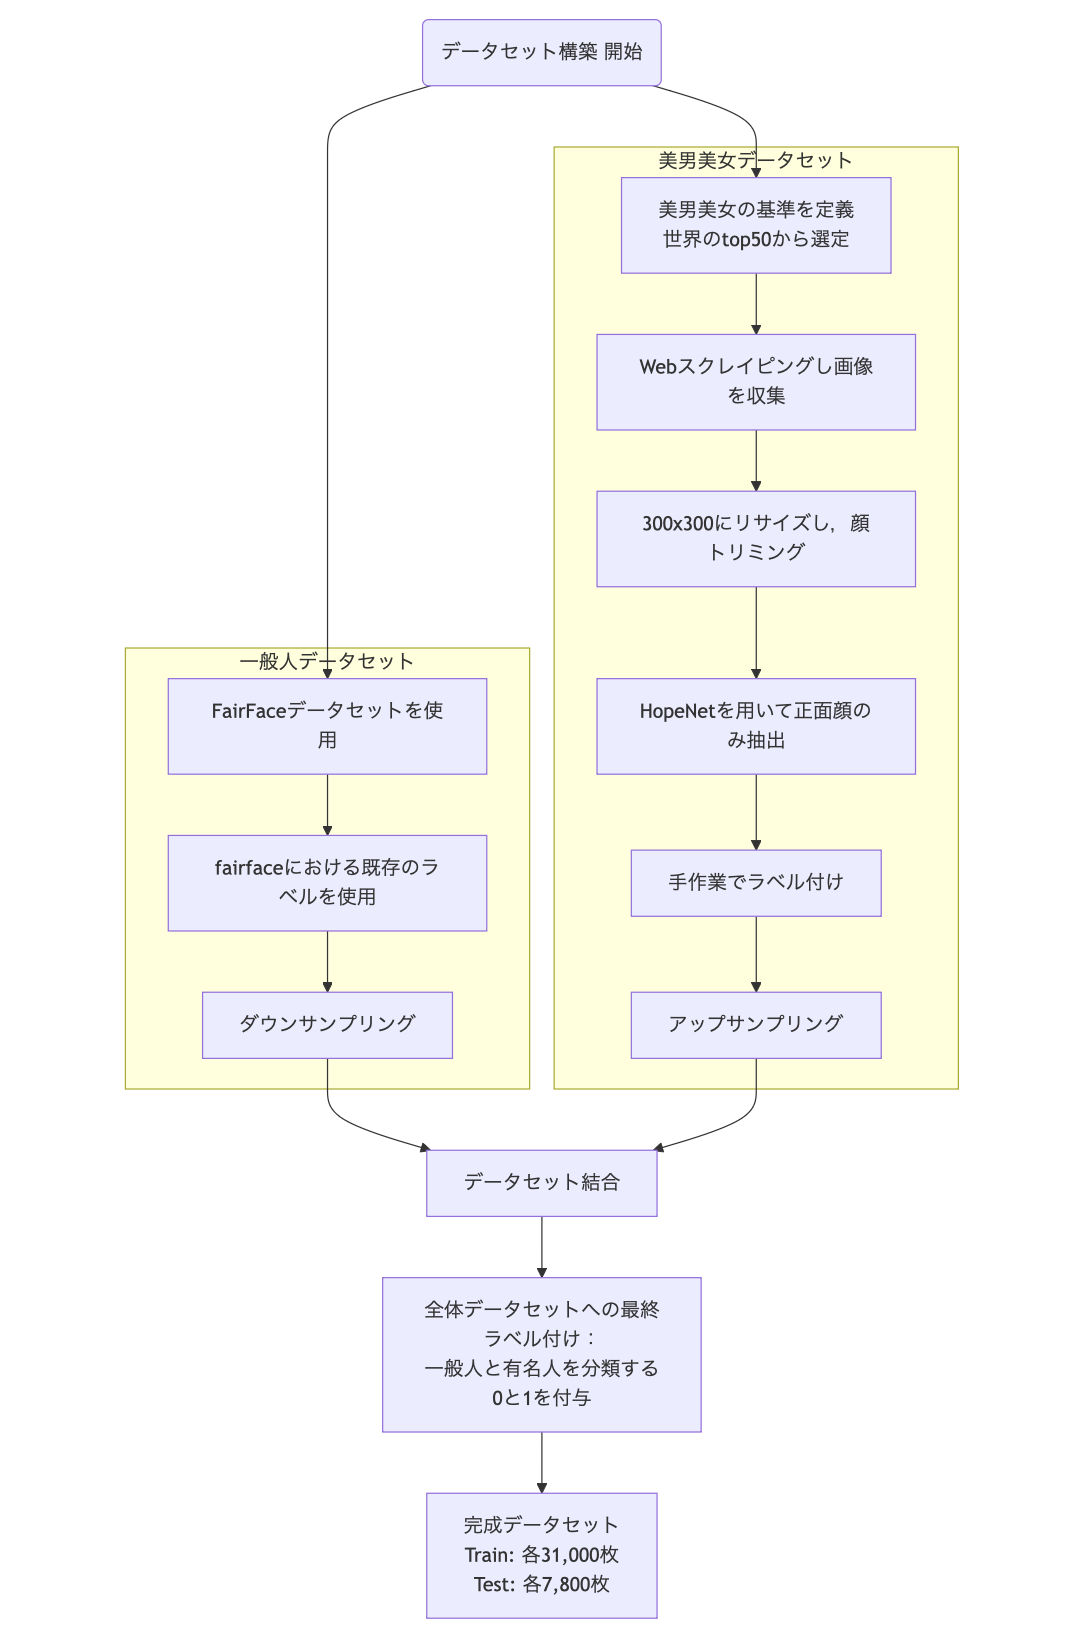
\includegraphics[width=0.9\textwidth]{final_rep_G1.png}
    \caption{前処理のフローチャート}
    \label{fig:csv}
\end{figure}
%======================


\subsection{モデル選定}
fairfaceが提供する学習済みモデルを本研究のタスクに合わせてカスタマイズした。これにはResNet34が使用されていたため,そのままResNet34を用いる。詳しくは\cite{karkkainenfairface}を参照されたい。\par
(後述するが,このfairfaceのカスタマイズモデルは精度が100\%になったため,別アプローチとして本実験ではfairfaceを用いず新規にResNet18, ResNet34, ResNet50も用いた。)


\subsection{パラメータ調整}
デフォルト値のまま使用している。

\section{実験}

\subsection{役割分担について}
\begin{itemize}
    \item 215706D:KIM HYUNWOO
        \begin{itemize}
            \item 正面画像抽出・ラベル付・複数のResNetとEfficientNetでの実行・Grad Cam
        \end{itemize}
    \item 235221E:山脇大輝
        \begin{itemize}
            \item FairFaceの調査,カスタマイズ,Webスクレイピング・リサイズ・トリミング・ラベル付
        \end{itemize}
    \item 235701B:松田遼平
        \begin{itemize}
            \item GitHubの操作補助
        \end{itemize}
    \item 235732B:長\UTF{7028}一生
        \begin{itemize}
            \item アップサンプリング・ダウンサンプリングコード作・背景のマスキング実施
        \end{itemize}
\end{itemize}

%\subsection{実験設計}
%\begin{itemize}
%    \item 実験の目標
%    \item 目標をどのように達成しようとしたのか
%\end{itemize}


\subsection{用意したデータセット画像}
図\ref{fig:good_ex},図\ref{fig:normal_ex}に用意したデータセットの画像の一部を示す。これは筆者がランダムに選択したものであり,レポートの可読性を向上させるために用意した。
%======================
\begin{figure}[htbp]
    \centering
    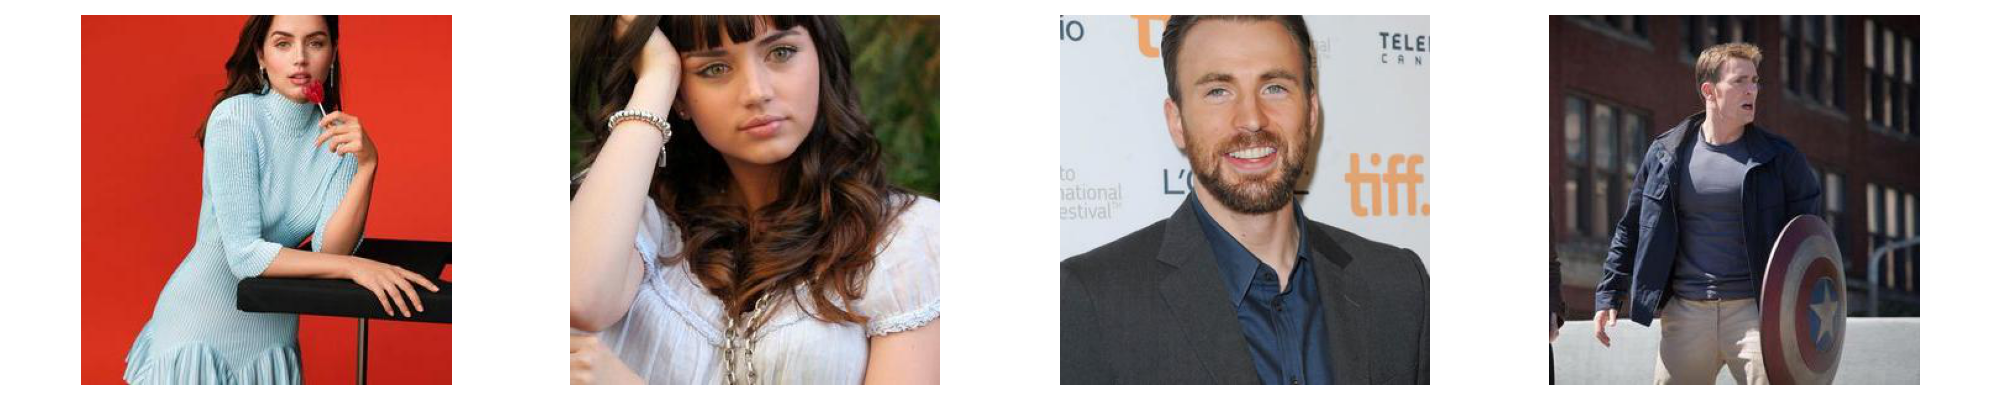
\includegraphics[width=1.1\textwidth]{ex_good_dataset.png}
    \caption{有名人データセットの画像例}
    \label{fig:good_ex}
\end{figure}
%======================
%======================
\begin{figure}[H]
    \centering
    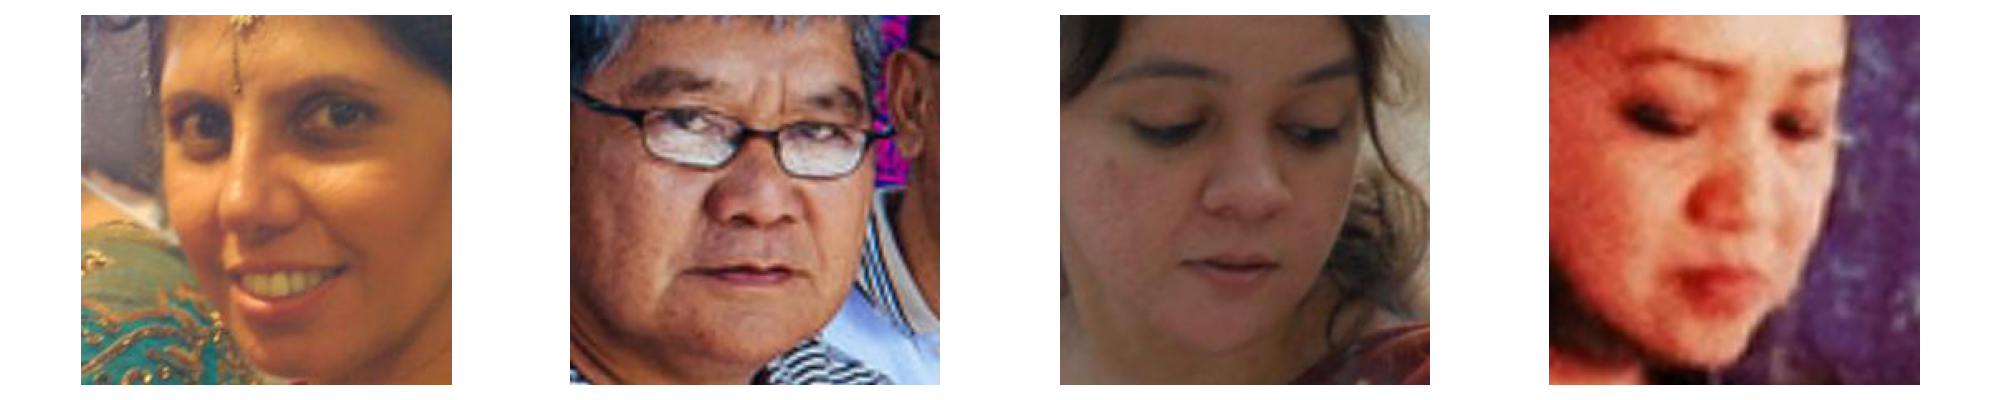
\includegraphics[width=1.1\textwidth]{ex_normal_dataset.png}
    \caption{一般人データセットの画像例}
    \label{fig:normal_ex}
\end{figure}
%======================


\section{実験結果}
% ここに実験結果を記述
fairfaceに追加学習をすることによって有名人と一般人の差異を明らかにすることであった。しかし,fairfaceに追加学習したモデル(custom)は精度が100\%になった。過学習の影響も考えられるが,fairfaceはそもそも学習済みモデルであり,本実験はこれに追加学習を行うアプローチのため原因の切り分けが困難である。\\
そこで,アプローチとしてResNet18,34,50とEfficientNetで新規に一般人と有名人の学習を行い,その結果を見る。




\section{失敗事例分析について:Grad-Camを用いたモデルの信頼性の検証}
Grad-CAM(Gradient-weighted Class Activation Mapping)というCNNが画像のどの部分に注目して一般人か美男美女かの判断を下したのかをヒートマップとして可視化する技術がある。
図\ref{fig:gradcam_good},図\ref{fig:gradcam_normal}にGrad-CAMを用いてモデルごとに有名人(good)と一般人(normal)の各データの平均したヒートマップを示す。

各画像は以下に示すモデルを適用した結果である。
\begin{itemize}
	\item 1行目
	\begin{itemize}
	\item 追加学習したモデル:custom
	\item EfficientNet\_b0
	\item ResNet18
	\end{itemize}
	\item 2行目
	\begin{itemize}
	\item ResNet34
	\item ResNet50
	\end{itemize}
\end{itemize}


	
%======================
\begin{figure}[htbp]
    \centering
    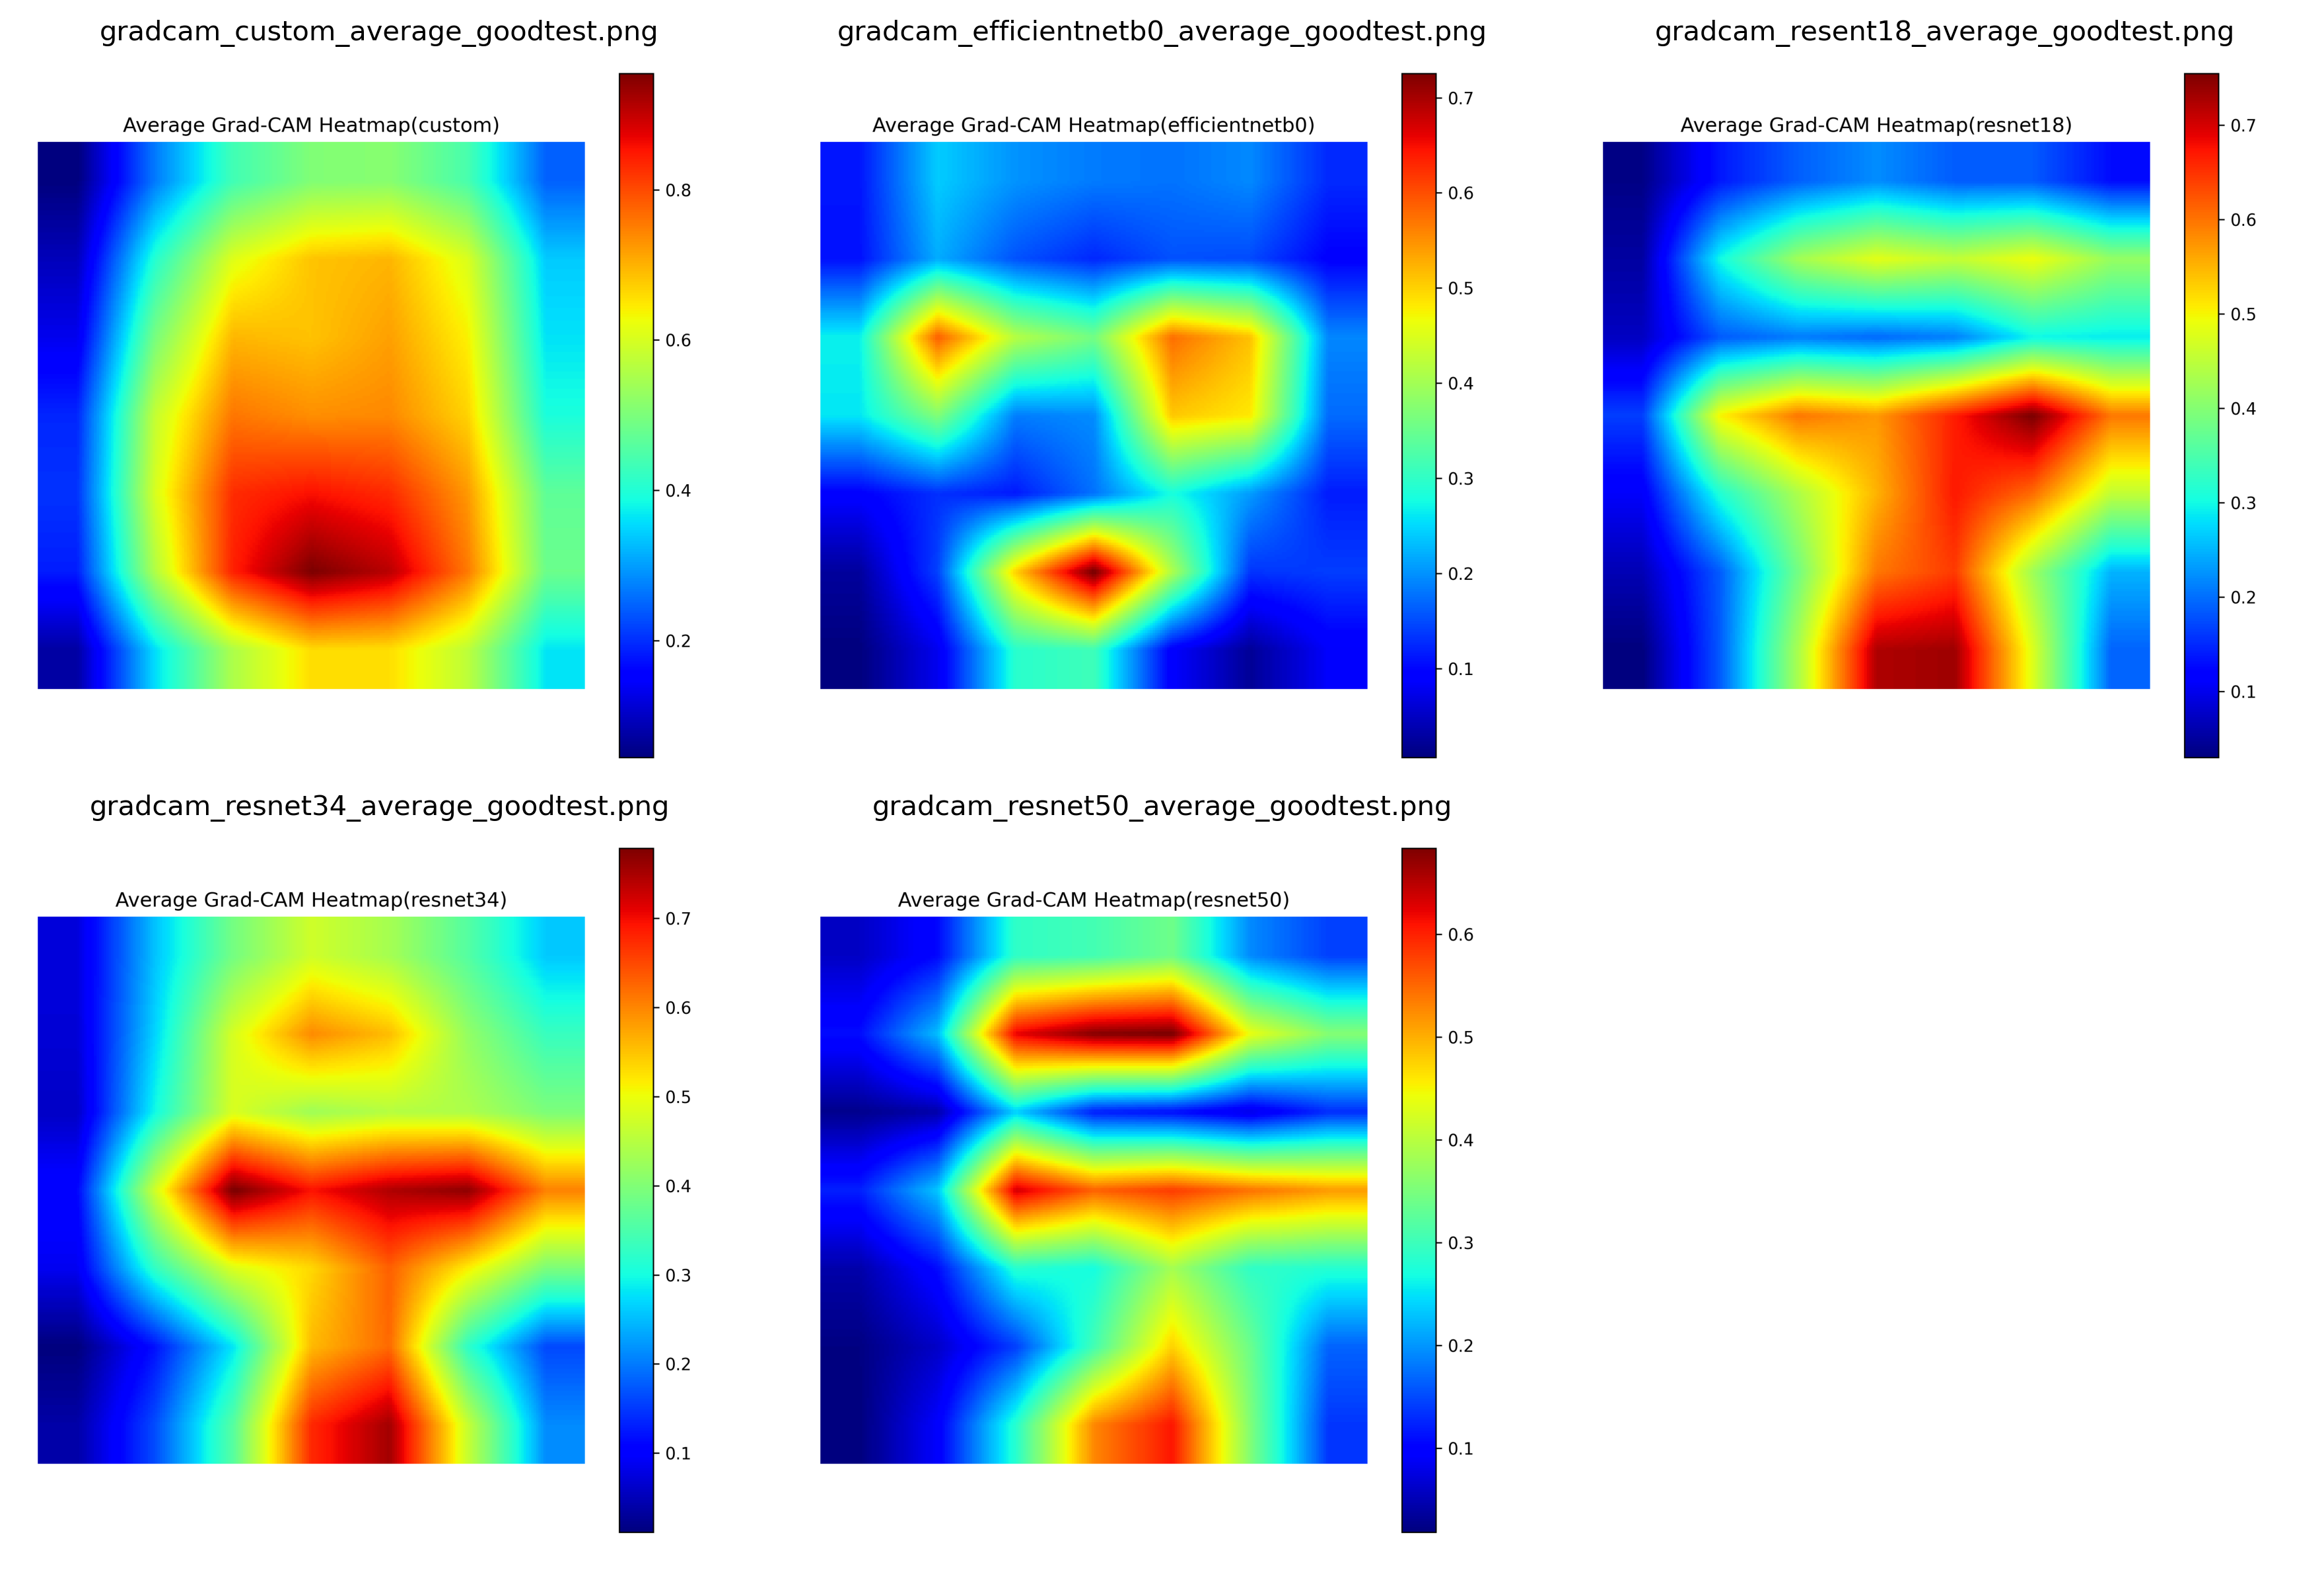
\includegraphics[width=1.1\textwidth]{combined_images_good.png}
    \caption{Grad-CAMを用いた有名人の判断根拠の可視化}
    \label{fig:gradcam_good}
\end{figure}
%======================
%======================
\begin{figure}[H]
    \centering
    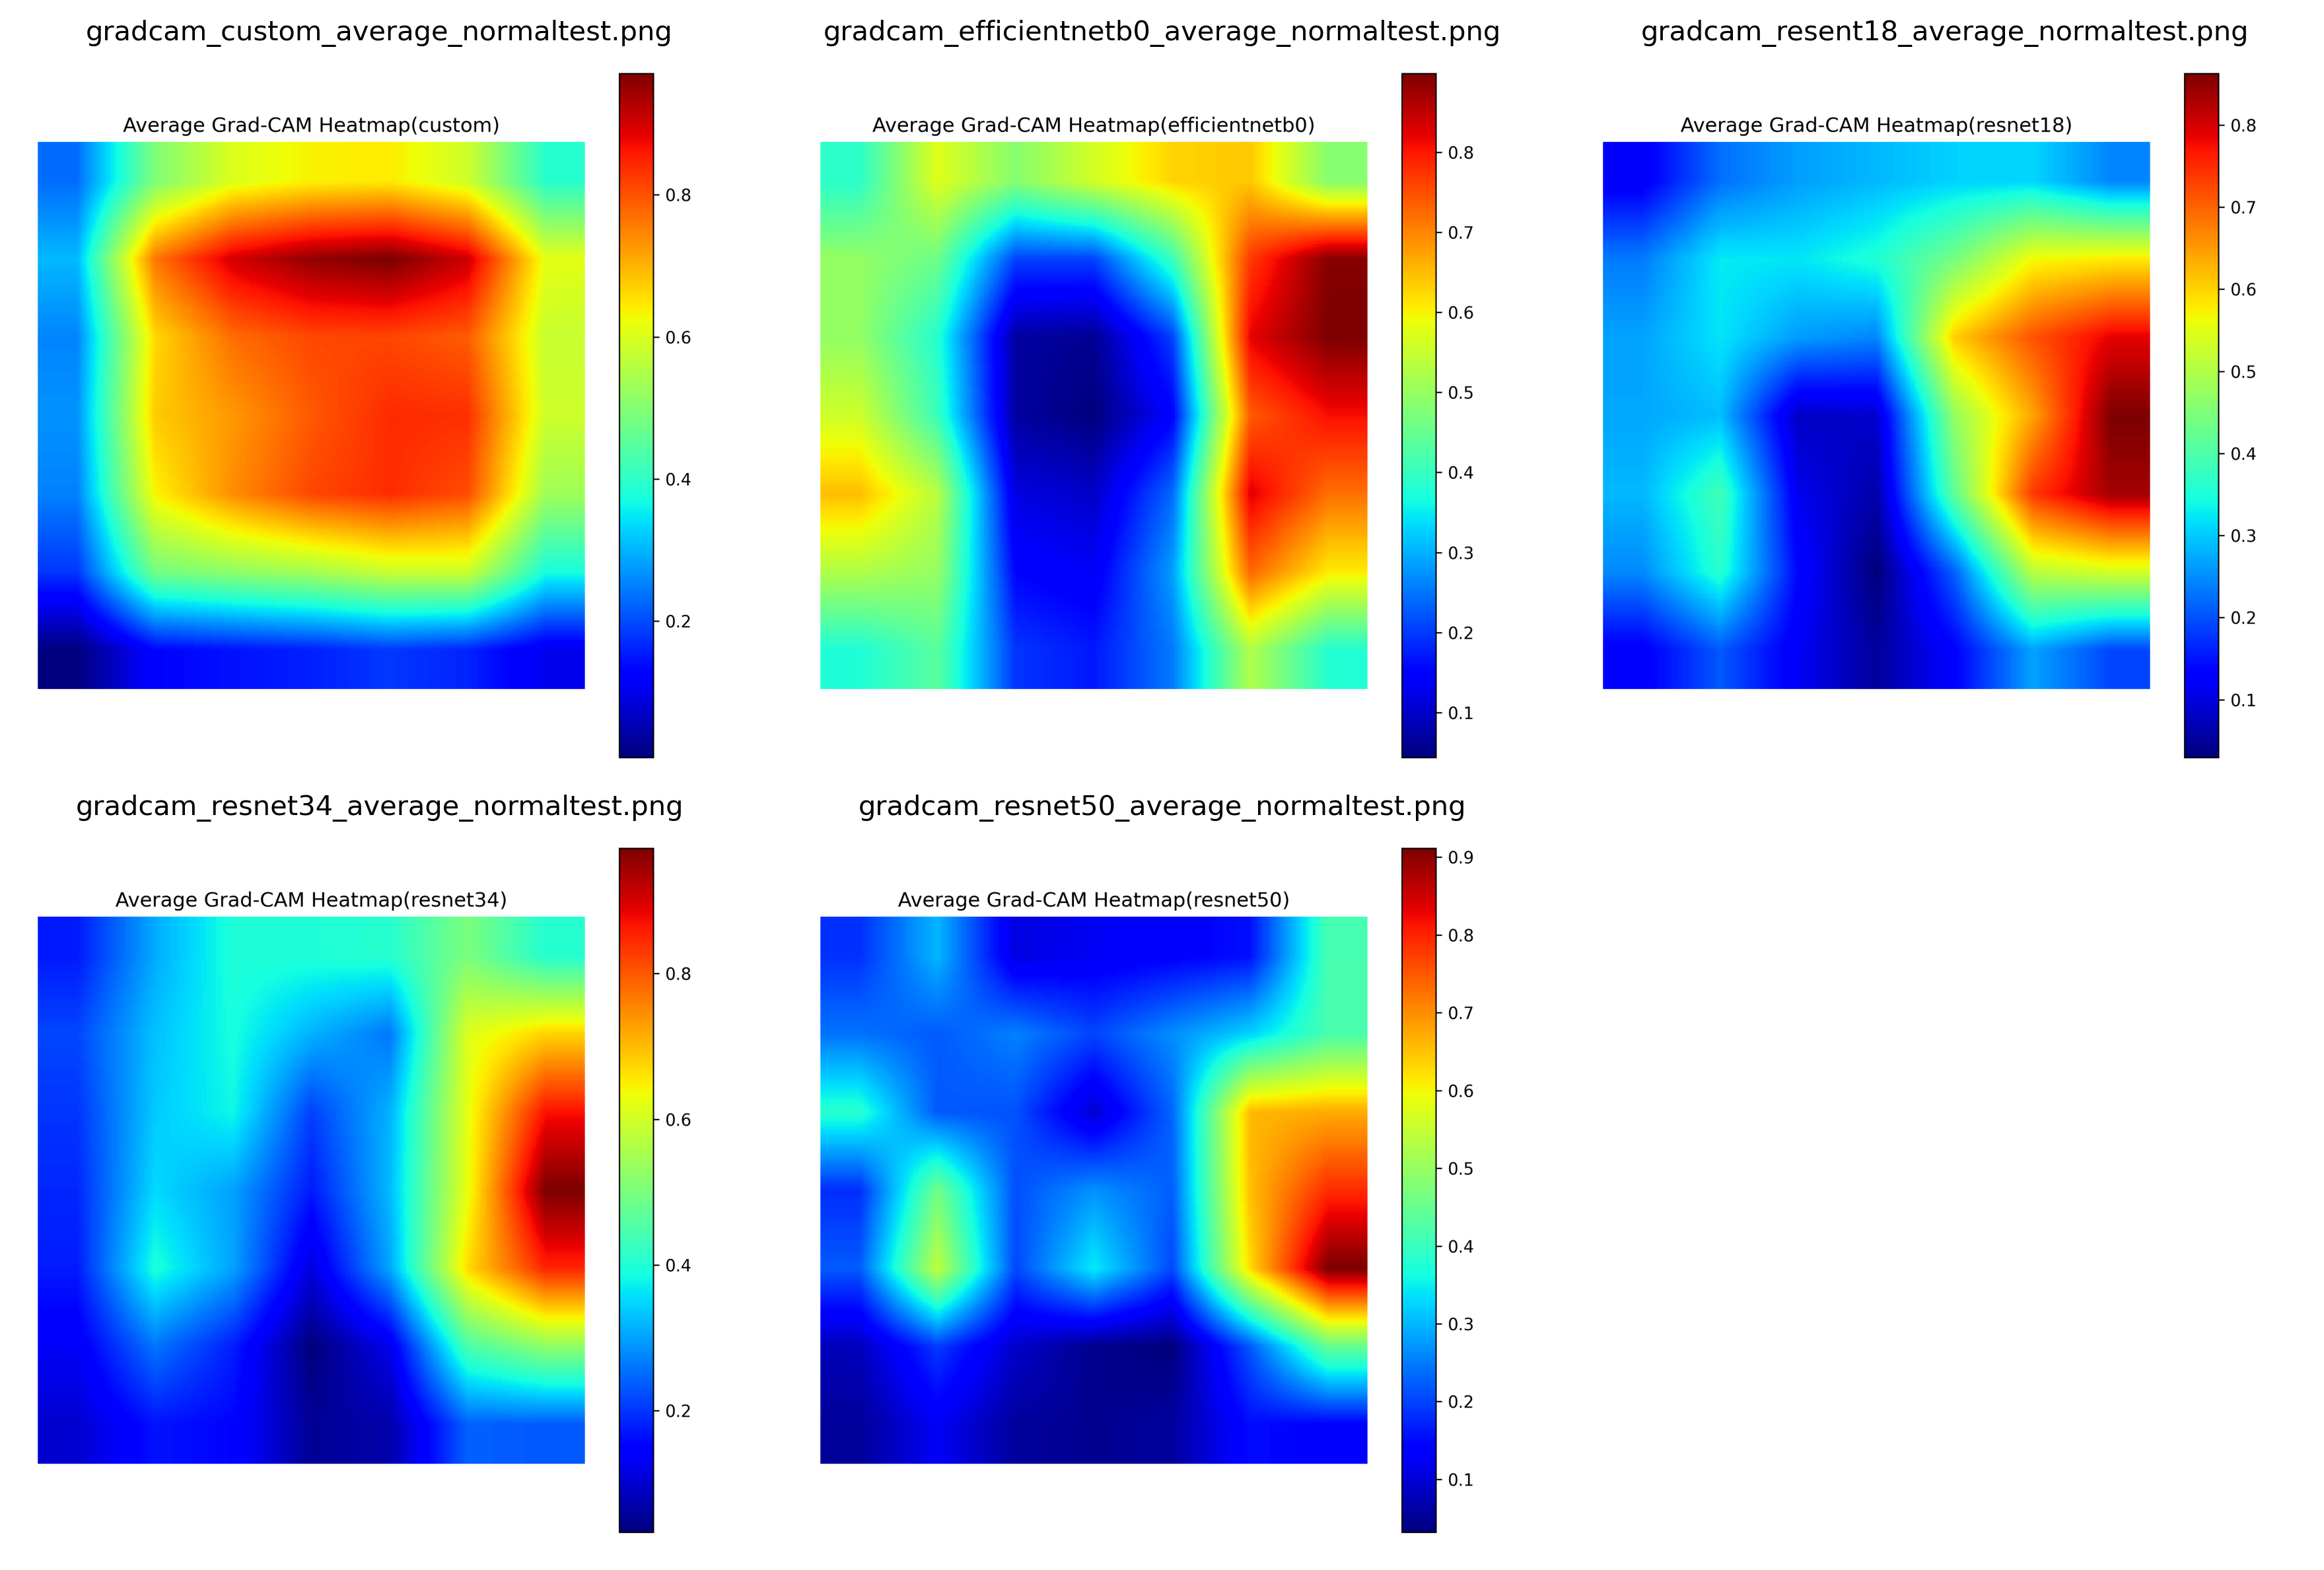
\includegraphics[width=1.1\textwidth]{combined_images_normal.png}
    \caption{Grad-CAMを用いた一般人の判断根拠の可視化}
    \label{fig:gradcam_normal}
\end{figure}
%======================


\subsection{実験結果の考察}
有名人の判断根拠について,customeは顔全体,特に口元がよく見られているが,それ以外のResNet・EfficientNetについては,全体の傾向として,目と口が判断根拠になっていることがわかる。\par
一方,一般人の判断根拠について,customモデルは目元の上部(額と思われる)を見ており,それ以外のモデルは人物の右背景を見ていることがわかる。右背景を見ているのでは目的であった顔を見て分類する目的を果たせておらず,実験の目標は達成できていない。
この原因については,図\ref{fig:good_ex},図\ref{fig:normal_ex}に示したように有名人の画像の全体的な傾向として,記者会見などで用いられるバックパネルやスタジオで撮影されていると思われる画像など,背景がシンプルなものが多い。一方で,一般人の画像は,Flickr 画像とTwitterやオンライン新聞の画像などがデータセットに使われており,人物の横に他の人の体の一部が写っていたりカメラを向いていなかったりするものが多い傾向にある。そういった構築したデータセットの画像の特徴から,一般人の分類において背景で判断されたと考えられる。そこで次の章では,画像を白背景にして再度を学習を行った。
%ただし,用意したデータセットをモデルごとに実行し,Grad-Camで得た出力の「モデルごとの平均」であることに注意したい。



\section{白背景画像を用いた失敗事例分析の改善}




\section{考察}
% ここに考察を記述

\section{反省・今後の課題}
githubを使おうとしたが,使える人数が少なくgithubでのバージョン管理が実質できていなかった。さらにamaneで実行する場合,さらにソースコードのバージョンが不透明になってしまった。
役割分担・実験計画が適切にできておらず,実験の後半で急いで学習を行った。計画よりも前処理に時間がかかり,その後も実行しその結果を考察する時間をファイルの欠損の対応・コンテナプラットフォームSingularity使用のための準備といった対応に終われてしまった。

\subsection{時間の都合上省いた項目}
\subsubsection{撮影日時による人物データの抽出}
画像をwebスクレイピングで収集したものについて,ネットに存在する有名人の画像は撮影された日時がバラバラである。若い時の写真もあれば現在の写真もあり,年齢によって発生する特徴量の変化については考慮できていない。検索キーワードをもとにスクレイピングをする際に,人名に年齢を含むアプローチも行ったが,得られる画像が少ない・検索してもそもそも年齢で絞れないという問題が発生した。本実験で調べる限りは実験の限界と判断し,他の前処理を丁寧に行う方を優先した。

\subsubsection{構築したデータセットの人名の偏り改善}
本実験では,2024年美男美女ランキングtop50をもとに,50名ずつ抽出し,アップサンプリング(左右反転)を施した。これは一般人のデータセットと比較して,偏りが生じる。他のアップサンプリングの方法として回転・輝度変更といった手法があるが,これらでさらにデータを増やすよりかは,美男美女の人名数を50名ずつよりさらに増やす方がバイアスを削減できると考える。本実験では時間の都合・第一回の実験時の計画がずれていたため省略した。

\section{まとめ}
fairfaceで構築されているデータセットは,本当にイケメンでない人が含まれているのかという疑問から,分担して画像を確認していったが,いわゆる芸能人並のイケメンの数は少なかった。


\begin{thebibliography}{9}
    \bibitem{karkkainenfairface}
    Karkkainen, Kimmo and Joo, Jungseock.
    FairFace: Face Attribute Dataset for Balanced Race, Gender, and Age for Bias Measurement and Mitigation.
    In \textit{Proceedings of the IEEE/CVF Winter Conference on Applications of Computer Vision}, pages 1548--1558, 2021.\\
        \url{https://arxiv.org/abs/1908.04913}
    
    \bibitem{bidanshi}
    Most Handsome Man In The World 2024, shiningawards.com, \\
    \url{https://shiningawards.com/most-handsome-man-in-the-world-2024/}
    
    \bibitem{bijoshi}
    Most Beautiful Faces 2024, gigazine.net, \\ \url{https://gigazine.net/gsc_news/en/20241229-most-beautiful-faces-2024/}
    
        \bibitem{hopenet}
        Nataniel Ruiz Eunji Chong and James M. Rehg (Georgia Institute of Technology).
        Fine-Grained Head Pose Estimation Without Keypoints
         In \textit{The IEEE Conference on Computer Vision and Pattern Recognition (CVPR) Workshops}, pages 2074--2083, 2018. \\
          \url{https://arxiv.org/abs/1710.00925}

    \bibitem{hopenet}
    Head Pose Estimation, \url{https://github.com/natanielruiz/deep-head-pose}
\end{thebibliography}

\end{document}